{\let\clearpage\relax\chapter*{Uzasadnienie wyboru tematu pracy}}
\addcontentsline{toc}{chapter}{Uzasadnienie wyboru tematu pracy}

Wraz z występującym w ostatnich latach systematycznym wzrostem liczby obrazowań medycznych uwidacznia się potrzeba na komputerowe wspomaganie pracy radiologów oceniających badania obrazowe. W szczególności zastosowanie znajdują aplikacje usprawniające generowanie raportów, rozwiązania do personalizacji diagnostyki i narzędzia poprawiające jej jakość.

Niniejsza praca, w odpowiedzi na powyższe zagadnienia, przedstawia propozycję strukturyzacji i automatyzacji oceny gojenia ścięgna Achillesa widocznego w obrazowaniu Rezonansem Magnetycznym (w skr. RM). Badanie to, w kontekście przedmiotowego ścięgna, jest dokładną metodą wykorzystywaną do oceny zmian strukturalnych i morfologicznych w zakresie tkanek miękkich. Wedle obecnych standardów ocena tego badania jest subiektywna i niesparametryzowana, a zatem stanowi ciekawy temat badawczy związany z możliwościami komputerowego wspomagania radiologów i usprawnienia ich pracy oraz w konsekwencji pomocy osobom ze schorzeniami ścięgna Achillesa.

Dodatkową motywację stanowi fakt dynamicznego rozwoju metod sztucznej inteligencji, a dokładniej ich podzbioru tj. głębokich sieci neuronowych, których rozwój znacząco przyspieszył od 2012 r. za sprawą innowacji w budowie sieci i szybkiej ewolucji możliwości sprzętowych. W szczególności konwolucyjne sieci neuronowe z uwagi na dużą skuteczność w problemach aplikowanych do przetwarzania obrazów znajdują zastosowanie w rosnącej liczbie narzędzi z certyfikacją medyczną dedykowanych dla radiologii.

Ograniczeniem wskazanych metod sztucznej inteligencji jest wymóg dużych, ustrukturyzowanych zbiorów danych, które mogą służyć do skutecznego uczenia się algorytmu. W toku prac nad wybraną problematyką, autor przedmiotowej rozprawy miał dostęp do unikatowego w skali światowej zbioru danych składającego się z 590 badań RM pacjentów po zerwaniu ścięgna Achillesa. Badania pochodziły z projektu START ("Wykorzystanie autologicznych mezenchymalnych komórek macierzystych w procesie regeneracji rekonstruowanego ścięgna Achillesa"), finansowanego przez Narodowe Centrum Badań i Rozwoju z krajowego programu STRATEGMED1.

Biorąc zatem pod uwagę występującą potrzebę w radiologii na wskazane innowacje, dynamiczny rozwój możliwości metod sztucznej inteligencji w tym zakresie i dostęp do zasobów umożliwiających realizację pierwszych w skali światowej badań nad możliwością strukturyzacji i automatyzacji oceny ścięgna Achillesa widocznego w badaniu RM, autor zdecydował się na wybór przedstawionej w pracy tematyki.  
 

{\let\clearpage\relax\chapter*{Cel i struktura pracy}}
\addcontentsline{toc}{chapter}{Cel i struktura pracy}

W ramach prac w projekcie START powstała koncepcja automatyzacji procesu monitorowania gojenia się ścięgna przy pomocy metod przetwarzania obrazów i sztucznej inteligencji. Założono, że głębokie sieci neuronowe będą skuteczne do oceny procesów patofizjologicznych widocznych w obrazowaniu medycznym takich jak gojenie tkanki miękkiej, co stanowi hipotezę przedmiotowej pracy.

Za cel główny autor postanowił obrać opracowanie automatycznej metody oceny gojenia się ścięgna Achillesa, natomiast cele poboczne stanowiły:
\begin{enumerate}[noitemsep,nolistsep]
	\item Wybór efektywnego kosztowo i czasowo protokołu badania bazującego na technikach obrazowania medycznego, a dokładniej Rezonansu Magnetycznego.
	\item Przetestowanie różnego rodzaju podejść związanych ze szkoleniem głębokich sieci neuronowych.
	\item Porównanie wyników oceny nowej metody z wynikami klasyfikacji bazującej na danych z ultrasonografii.
	\item Porównanie wyników oceny nowej metody z oceną funkcjonalną, rutynowo stosowaną do wspomagania rehabilitacji po urazie ścięgna.
\end{enumerate}

W celu uporządkowanego i zrozumiałego przedstawienia podłoża oraz wyników badań, w pracy wprowadzono podział na Rozdziały. Po wstępie i opisie celu pracy, w Rozdziale 3 zostały opisane współczesne metody monitorowania gojenia się ścięgna Achillesa. Rozdział ten rozpoczyna się od omówienia podstaw anatomicznych, biomechanicznych oraz dynamiki procesu gojenia się przedmiotowego ścięgna. Następnie przedstawiony jest szczegółowy opis badań obrazowych i biomechanicznych wykorzystywanych do oceny stanu rehabilitującego się pacjenta. 

W Rozdziale 4, omówione zostały szczegółowo konwolucyjne sieci neuronowe, które posłużyły jako rdzeń opracowanego rozwiązania. W szczególności, w opisie uwzględniono problemy z budową efektywnych modeli na bazie sieci neuronowych. 

W Rozdziale 5 zaprezentowano nowatorską metodę automatycznej oceny procesu gojenia się ścięgna Achillesa. Co istotne, omówiono unikatowy zbiór danych oraz wzorzec odniesienia, dzięki którym możliwa była realizacja przewidzianych badań i walidacja metody. Przedstawiono również eksperymenty wykorzystane do doboru komponentów i parametrów ostatecznego modelu oraz finalny wynik funkcjonowania opracowanego algorytmu. 

W Rozdziale 6 opisano zestawienie wyników metody z wynikami oceny realizowanej przez inne podejścia. W szczególności porównano przedmiotową metodę z metodą uczącą się explicite modelować ocenę radiologa, opracowaną również pod kierownictwem autora tej pracy w ramach pobocznych działań. Następnie zaprezentowano zestawienie z wynikami metody działającej w oparciu o dane z ultrasonografii, również opracowanej pod kierownictwem autora tej pracy. Finalnie, porównano wyniki z oceną biomechaniczną realizowaną standardowo przez fizjoterapeutów. Wnioski z porównań natury praktycznej spisano w Rozdziale 7. Całość pracy zakończono podsumowaniem przedstawionym w Rozdziale 8.

{\let\clearpage\relax\chapter*{Zbiór danych}}
\addcontentsline{toc}{chapter}{Zbiór danych}

W ramach projektu przebadano 59-ciu pacjentów po całkowitym zerwaniu ścięgna Achillesa i 27-ciu ochotników. Kryteria kwalifikacji i szczegóły dotyczące urazów opisano w pracy.

Podczas trwającej 12 miesięcy rehabilitacji pacjenci byli monitorowani z wykorzystaniem RM GE Signa HDxt 1.5T wyposażonego w cewkę Foot \& Ankle dedykowaną do pomiarów w rejonie dolnej kończyny. Każde z badań RM było wykonane z użyciem 7-miu sekwencji i łącznie 10-ciu modalności.

W grupie zdrowych ochotników przeprowadzono pojedyncze badanie, natomiast pacjentów skanowano 10-krotnie w odpowiednio zdefiniowanych odstępach czasowych. Pierwsze badanie odbyło się przed operacją, a następnych 9 odpowiednio w tygodniach: 1, 3, 6, 9, 12, 20, 26, 40 i 52 po operacji. Zbiory trójwymiarowe posłużyły do przygotowania dwuwymiarowych danych wejściowych dla wykorzystanych architektur sieci neuronowych. Finalna liczba tak utworzonych obrazów wyniosła 11.725 (oznaczonych jako obrazy zdrowego ścięgna) i 138.604 (oznaczonych jako obrazy chorego ścięgna). W zależności od wymogów eksperymentu liczby te były zmniejszane poprzez próbkowanie lub sztucznie powiększane z wykorzystaniem metod augmentacji danych.

Dodatkowo zgromadzono ustrukturyzowany opis radiologiczny dla 48-miu pacjentów w 10 krokach czasowych (480 ankiet z 6-cioma parametrami ocenionymi w skali 0--7). Czterech pacjentów (40 badań) zostało losowo wydzielonych na początku eksperymentów jako pacjenci testowi wykorzystani do celów wnioskowania i porównań wyników badań.

{\let\clearpage\relax\chapter*{Nowa metoda oceny ścięgna Achillesa}}
\addcontentsline{toc}{chapter}{Nowa metoda oceny ścięgna Achillesa}

W wyniku prac została opracowana komputerowa metoda oceny ścięgna Achillesa widocznego w badaniach RM, generująca numeryczny wynik w skali 0--7 dla 6-ciu zdefiniowanych w ramach projektu START radiologicznych parametrów opisujących strukturę i morfologię tkanek miękkich. Schemat generacji wartości pojedynczego parametru ilustruje rysunek poniżej. 
\begin{figure}[h!]
	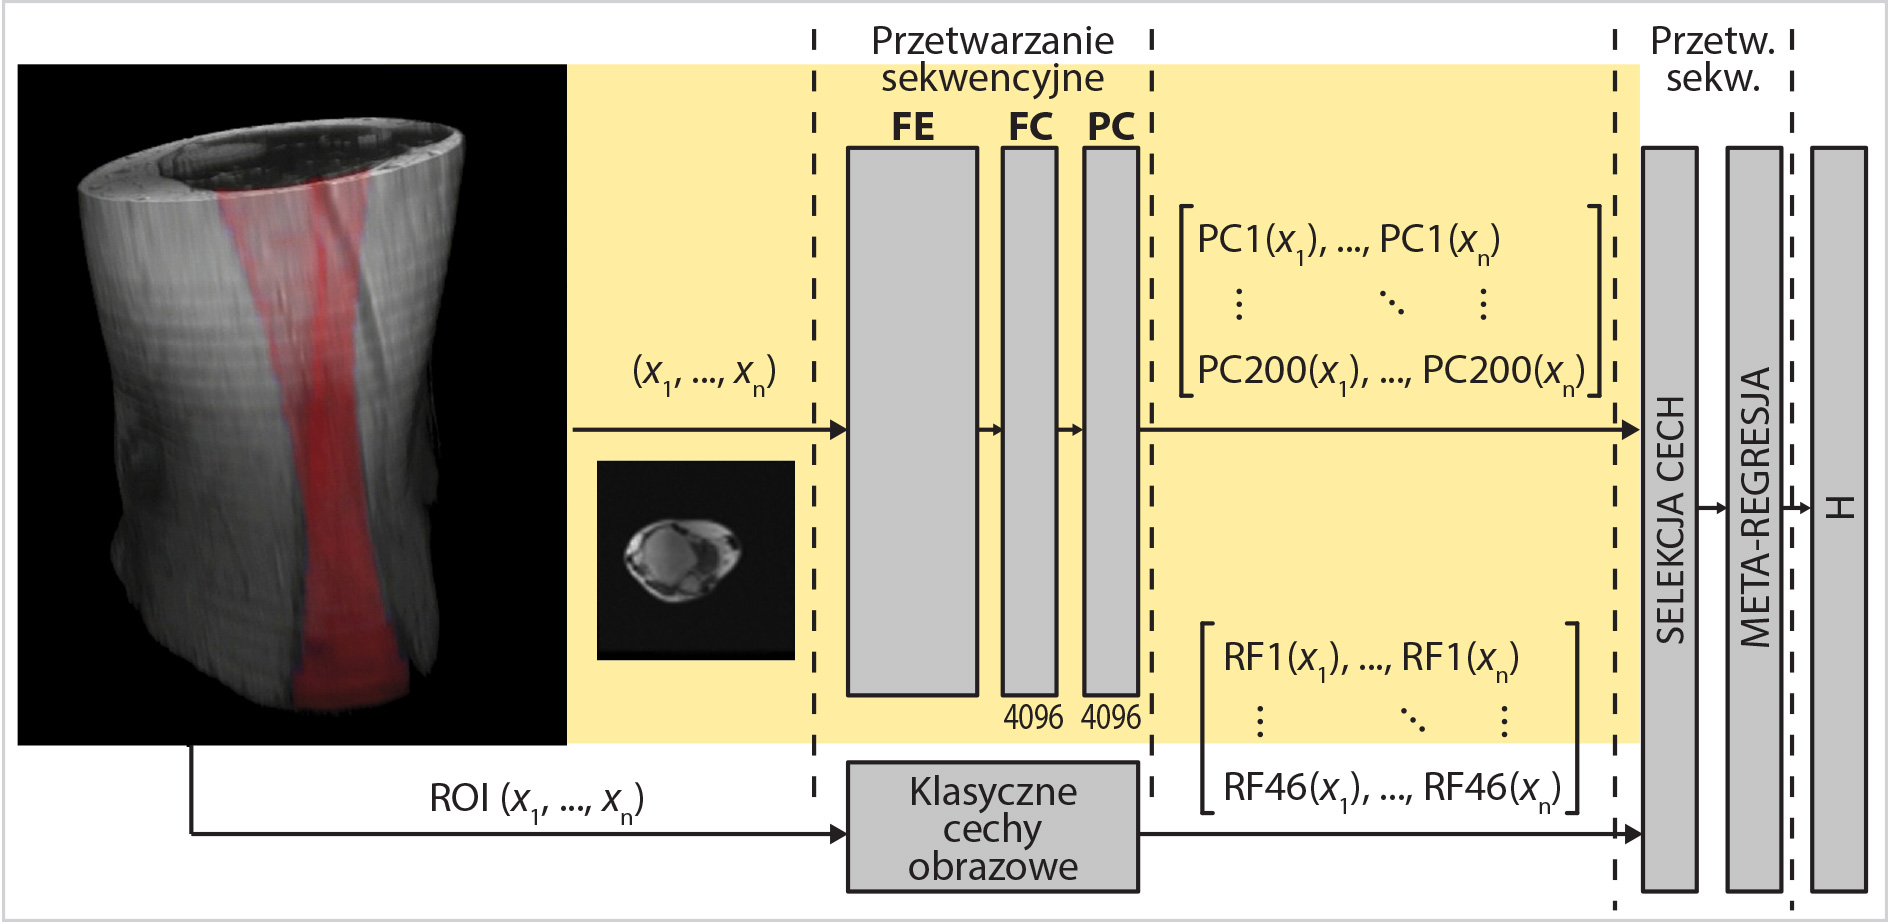
\includegraphics[width=\textwidth]{figures/net.jpg}
	\caption{Schemat automatycznej metody oceny pojedynczego parametru procesu gojenia się ścięgna Achillesa.} \label{fig:net}
\end{figure}

Dane wejściowe stanowi trójwymiarowe badanie RM obszaru podudzia. Badanie dzielone jest na $n$ obrazów będących przekrojami poprzecznymi względem osi długiej ścięgna. Z każdego przekroju dwojako ekstrahowane są zestawy cech. Po pierwsze, wykorzystywany jest ekstraktor cech będący złożeniem warstw konwolucyjnych i jednej warstwy gęstej wytrenowanej sieci neuronowej na wyjściu (po redukcji z wykorzystaniem metody analizy czynników głównych) generującej 200 wartości. Po drugie, dla obszaru ścięgna widocznego na każdym z przekrojów, wyliczane są cechy statystyczne i teksturalne, których łączna liczba wynosi 46. Z pośród tak utworzonego zestawu 246 wartości, dla każdego z 6-ciu radiologicznych parametrów, wybierane są z wykorzystaniem metody LASSO optymalne podzbiory o liczebności mniejszej niż 20. Podzbiory są kolejno procesowane z wykorzystaniem regresji opartej o algorytm wektorów nośnych, której wyniki dla poszczególnych przekrojów łączone są z wykorzystaniem średniej trymowanej odrzucającej rezultaty skrajne i generującej pojedynczą wartość parametru dla całego badania 3D RM.   


{\let\clearpage\relax\chapter*{Charakterystyka i wyniki przeprowadzonych badań}}
\addcontentsline{toc}{chapter}{Charakterystyka i wyniki przeprowadzonych badań}

Eksperymenty podzielono na dwa etapy. W pierwszym zrealizowano zagadnienia związane z doborem parametrów komponentów nowej metody i oceną jej skuteczności działania. W drugim porównano skuteczność nowej metody z innymi koncepcjami oceny gojenia ścięgna Achillesa. 

W ramach pierwszego etapu wyłoniono, z pośród 10-ciu modalności RM analizowanych w pracy, jedną sekwencję będącą najlepszym kandydatem na dane wejściowe. W tym celu zrealizowano zarówno badania związane z analizą wizualną jak i testami ilościowymi. Wybrana sekwencja to T2$^\ast$ GRE TE\_MIN, w której obraz ścięgna najlepiej różnicuje etapy gojenia się. Taki proces widoczny jest na rysunku poniżej.
\begin{figure}[h]
	\centering
	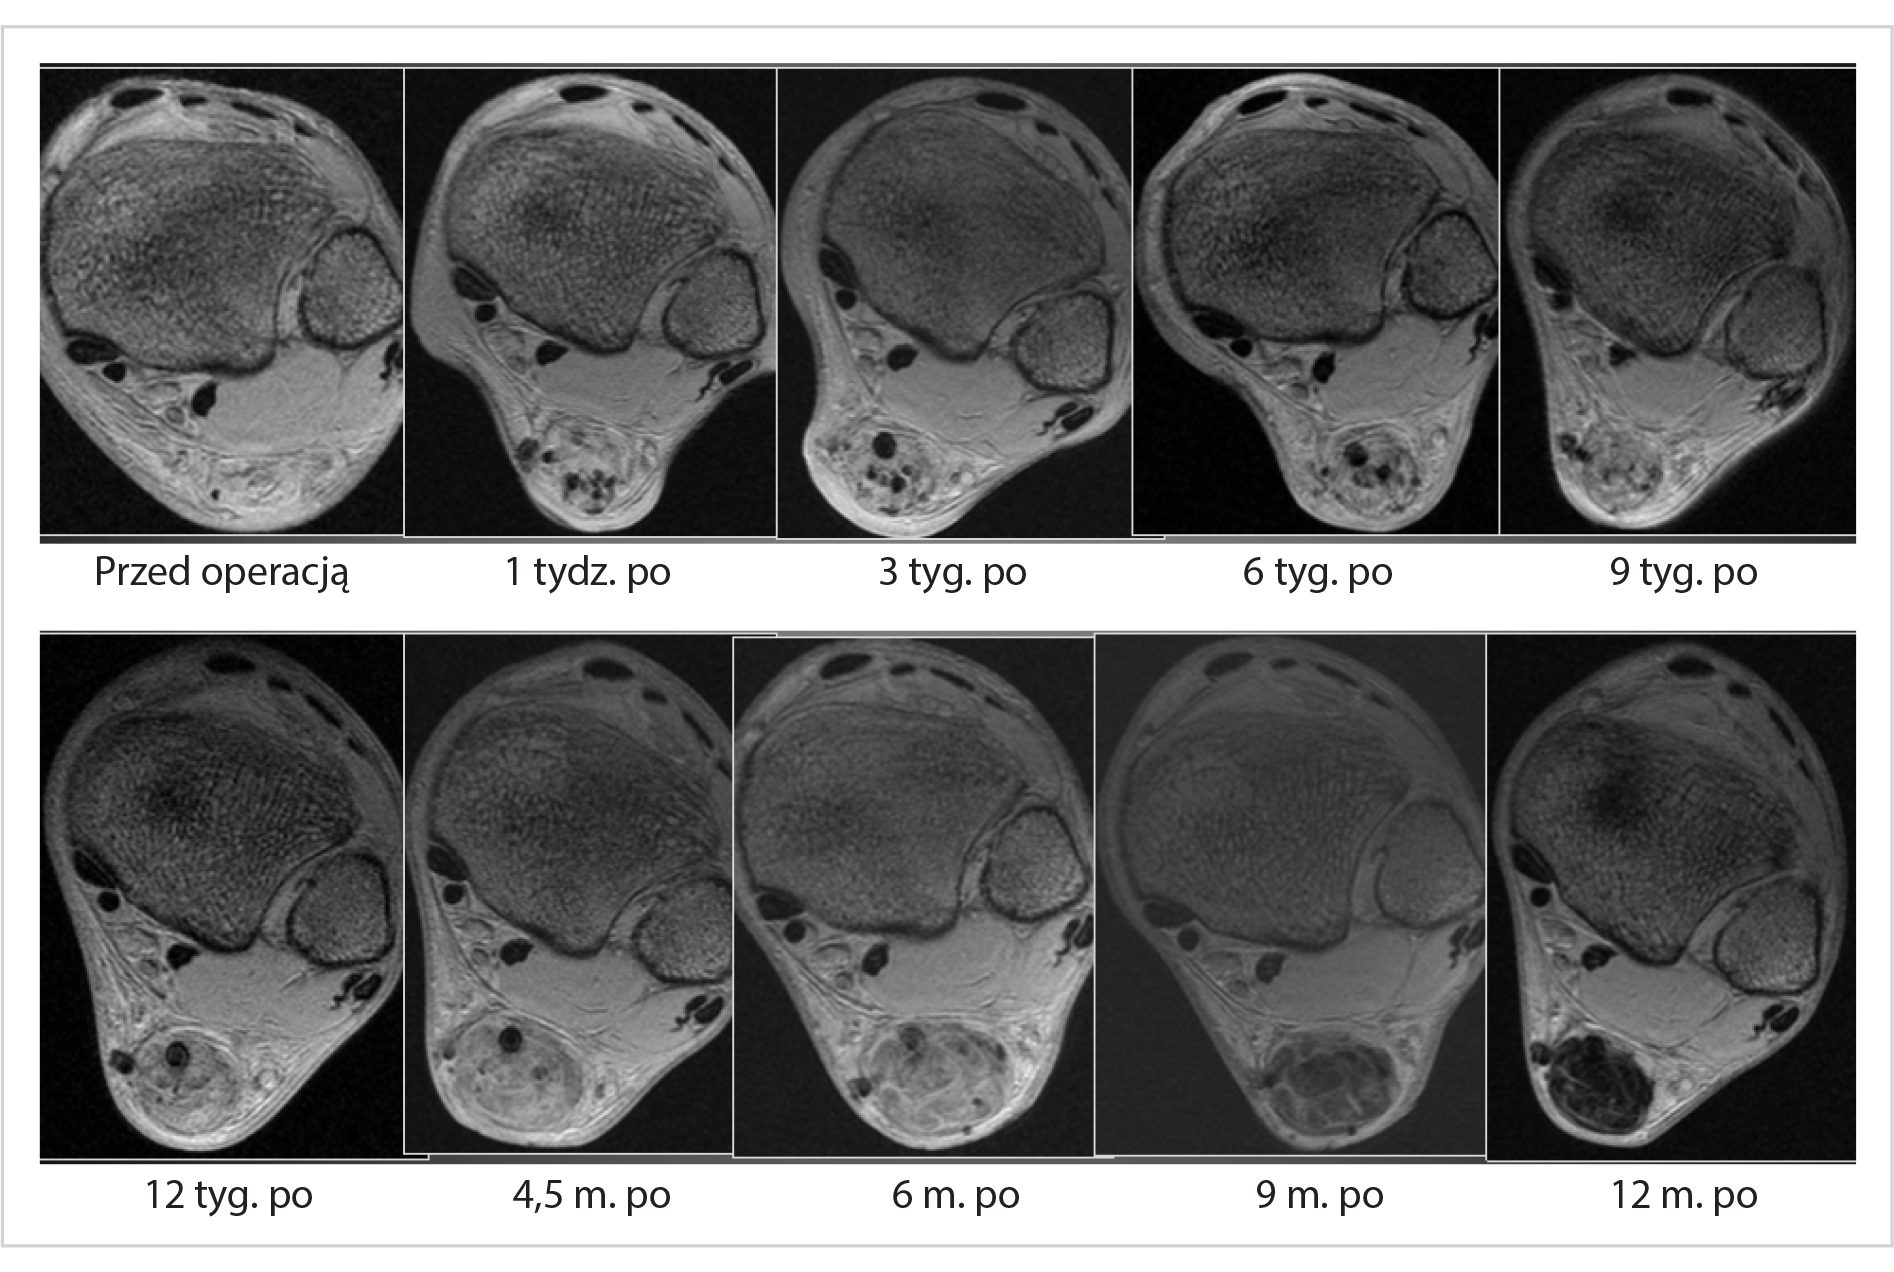
\includegraphics[width=1\textwidth]{figures/T2gremin.jpg}
	\caption{Proces gojenia się ścięgna Achillesa widoczny w obrazach zrekonstruowanych na podstawie danych z sekwencji T2$^\ast$ GRE TE\_MIN.}\label{fig:T2comp}
\end{figure}

Na przestrzeni całego procesu gojenia się ścięgna, zmiany uwidaczniają się w postaci silnie rozróżnialnych odcieni szarości w obszarze ścięgna, co nie występuje w innych sekwencjach.
Jednocześnie zbadano, iż dodawanie kolejnych sekwencji nie miało istotnie statycznego wpływu na polepszenie jakości predykcji wartości parametrów radiologicznych, a skutkowało wydłużeniem czasu badania pacjenta. 

W ramach badań nad doborem parametrów nowej metody, po pierwsze, zrealizowano wyliczenie parametrów ekstraktora cech poprzez zadanie treningu z celem binarnego podziału obrazów pacjentów na zdrowe i chore ścięgna. Przetestowano 3 architektury sieci neuronowych i na podstawie analizy ich dokładności klasyfikacji oraz czasu treningu wybrano sieć AlexNet. Takie podejście umożliwiło zakodowanie w ekstraktorze charakterystycznych cech dla tkanki zdrowej i patologicznej oraz finalne pogrupowanie ich w wektor o wymiarze 4096. Analiza tego wektora dla 10-ciu wybranych losowo pacjentów, uwidoczniła możliwość redukcji do 200 czynników głównych z zachowaniem blisko 99\% poziomu wariancji. W kolejnym kroku podjęto próbą fuzji tych cech z 46-cioma cechami wybranymi na podstawie analizy literatury, ekstrahowanymi z obszaru ścięgna. W tym celu wykorzystano własność metody LASSO związaną z zerowaniem się współczynników mających marginalny wpływ na ostateczny wynik zadania. Zrealizowano badanie, dla którego wyniki metody LASSO (tj. błąd średniokwadratowy powiększony o funkcje kary) dla każdego pacjenta zestawiono w krzywe łączące kolejne punkty obrazowania. Kryterium selekcji współczynników była najlepsza korelacja wzorca odniesienia z krzywymi, którą uzyskano dla $\alpha$ = 0,1. W rezultacie, dla 6-ciu parametrów wzorca odniesienia uzyskano różnicujące podzbiory $n$ predyktorów, gdzie $n<$ 20. Wykorzystując podzbiory i stosując metodę generalizacji stosów (stacking) wytrenowano oraz porównano szereg meta-regresorów: maszynę wektorów nośnych, wielowarstwowy perceptron, drzewa losowe jak i regresję liniową oraz nieliniową. W wyniku badania wybrano algorytm bazujący na wektorach nośnych, który dla każdego przekroju badania 3D oblicza ocenę z zakresu 0--7 dla zadanego parametru radiologicznego. Dla finalnej oceny badania 3D wybrano prostą metodę uśrednienia z odrzuceniem wartości skrajnych ocen poszczególnych przekrojów. 

Opracowaną metodę (SVR) zwalidowano z wykorzystaniem zbioru testowego tj. 4-ech pacjentów (40 badań). Do oceny wykorzystano miary średniego błędu absolutnego (MAE) z informacją na temat błędu średniej, maksymalnego błędu absolutnego (MAX-AE) i średniej korelacji obliczonej z wykorzystaniem transformacji Z-Fishera (Corr). Ocenę wykonano dla wszystkich sześciu parametrów radiologicznych o nazwach: SCT, TT, STE, TE, TU, TisE. Szczegóły znajdują się w tabeli poniżej.

\begin{table*}[]
	\caption{Wyniki oceny procesu gojenia z wykorzystaniem proponowanej metody.}
	\scriptsize
	\begin{center}
		\begin{tabular}{lc||c|c|c|c|c|c}
			\textbf{Model} & & \textbf{SCT} & \textbf{TT} & \textbf{STE} & \textbf{TE} & \textbf{TU} & \textbf{TisE}\\ 
			
			\hline \hline
			\multirow{3}{*}{SVR}
& MAE & 1,05$\pm0,06$ & $0,56\pm0,03$ & $0,75\pm0,04$ & $0,91\pm0,05$ & $0,91\pm0,04$ & 0,94$\pm0,05$\\
& MAX-AE & 2,62 & 1,82 & 1,92 & 2,54 & 2,01 & 2,38 \\
& Corr   & 0,85 & 0,85 & 0,31 & 0,72 & 0,65 & 0,80 \\
\hline
		\end{tabular}
	\end{center}
	\label{tab:trainset}
\end{table*}

Dla każdego z pacjentów testowych przeanalizowano również krzywe gojenia, których przykład znajduje się na rysunku poniżej.

\begin{figure}[h!]
	\centering
	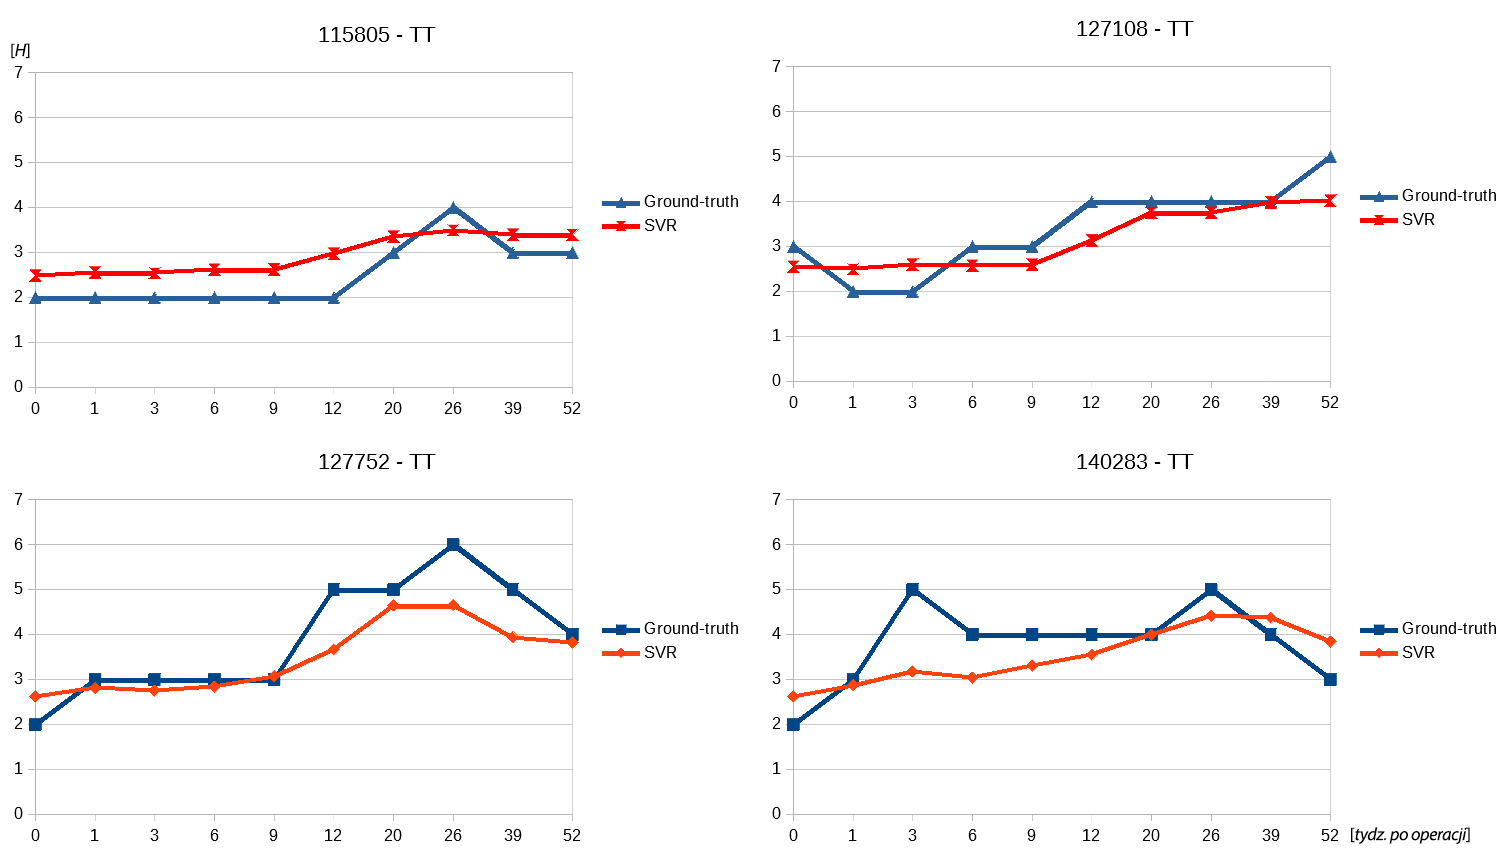
\includegraphics[width=1\textwidth]{figures/TT.png}
	\caption{Ocena parametru TT.}\label{fig:TT}
\end{figure}

Nową metodę porównano z dwiema innymi propozycjami oceny gojenia się ścięgna opracowanymi w grupie pod kierownictwem autora tej rozprawy, który odpowiadał za sformułowanie założeń eksperymentów i ich analizę, oraz z metodą bazującą na testach biomechanicznych realizowaną u partnera klinicznego. Pierwsze dwa podejścia wytrenowano w koncepcji end-to-end tak, aby modelowały \textit{explicite} ocenę radiologa wykorzystując (1) poetykietowane obrazu RM, (2) poetykietowane obrazy ultrasonografii (USG). Wyniki przedstawione są w tabeli poniżej.

\renewcommand{\arraystretch}{1.2}
\begin{table*}[h]
	\caption{Porównanie wyników wnioskowania z wykorzystaniem zbioru testowego dla metody proponowanej tj. SVR oraz metody wyszkolonej w paradygmacie end-to-end. Pogrubieniem oznaczono najlepsze rezultaty, a kolorem czerwonym istotne statystycznie różnice w liczonych średnich ($p$ $<$ 0,05).}
	\scriptsize
	\begin{center}
		\begin{tabular}{lc||c|c|c|c|c|c}
			\textbf{Model} & & \textbf{SCT} & \textbf{TT} & \textbf{STE} & \textbf{TE} & \textbf{TU} & \textbf{TisE}\\ \hline \hline
			Inception-v3$_{e}$ & MAE & 1,12$\pm{0,08}$ & 0,80$\pm{0,04}$ & 1,40$\pm{0,07}$ & \textbf{0,89}$\pm{0,05}$ & 1,08$\pm{0,04}$ & \textcolor{red}{\textbf{0,69}}$\pm{0,07}$ \\
			& MAX-AE & \textbf{2,14} & \textbf{1,01} & 2,13 & \textbf{1,18} & \textbf{1,44} & \textbf{0,78} \\
			& Corr & 0,82 & 0,77 & 0,05 & 0,59 & 0,52 & 0,77 \\ \hline
			SVR & MAE & \textbf{1,05}$\pm0,06$ & \textcolor{red}{\textbf{0,56}}$\pm0,03$ & \textcolor{red}{\textbf{0,75}}$\pm0,04$ & 0,91$\pm0,05$ & \textcolor{red}{\textbf{0,91}}$\pm0,04$ & $0,94\pm0,05$\\
			& MAX-AE & 2,62 & 1,82 & \textbf{1,92} & 2,54 & 2,01 & 2,38 \\
			& Corr & \textbf{0,85} & \textbf{0,85} & \textcolor{red}{\textbf{0,31}} & \textcolor{red}{\textbf{0,72}} & \textcolor{red}{\textbf{0,65}} & \textbf{0,80} 
		\end{tabular}
	\end{center}
	\label{tab:end-to-end_testset}
\end{table*}
\renewcommand{\arraystretch}{1}

\renewcommand{\arraystretch}{1.2}
\begin{table}[h]
	\scriptsize
	\setlength{\tabcolsep}{1pt}
	\centering
	\caption{Porównanie wyników oceny automatycznej, bazującej na danych USG i RM, dla pacjentów ze zbioru testowego. Pogrubieniem oznaczono najlepsze wyniki. Kolorem czerwonym oznaczono poprawę w stosunku do kolejnego wyniku istotną statystycznie z $p$ $<$ 0,05.}
	\label{tab:USGvsRM-cross-validation}
	\vspace{-0.5cm}
	\begin{tabular}{lc||c|c|c|c|c|c}
		%\hline
		& & \multicolumn{6}{c}{\textbf{USG -- p. strzałkowy}} \\
		\textbf{Model} & & \textbf{SCT} & \textbf{TT} & \textbf{STE} & \textbf{TE} & \textbf{TU} & \textbf{TisE} \\ \hline \hline
		Inception-v3$_{eus}$ & MAE & \textbf{0,81}$\pm$0,19 & 0,63$\pm$0,03 & \textbf{0,56}$\pm$0,09 & 0,85$\pm$0,10 & 0,54$\pm$0,02 & 0,87$\pm$0,14 \\
		& MAX-AE & 1,59 & 1,79 & 1,7 & \textbf{1,25} & \textbf{1,38} & 1,69 \\
		& Corr & 0,80 & 0,77 & 0,31 & 0,52 & \textbf{0,69} & 0,62 \\ \hline
		ResNet-50$_{eus}$ & MAE & 0,88$\pm$0,16 & 0,65$\pm$0,07 & 0,66$\pm$0,04 & 0,83$\pm$0,12 & 0,75$\pm$0,06 & 0,93$\pm$0,11 \\
		& MAX-AE & \textbf{1,49} & \textbf{1,26} & 1,74 & 1,48 & 1,78 & 1,71 \\
		& Corr & 0,60 & 0,55 & 0,25 & 0,55 & 0,34 & 0,56 \\
		\hline \hline
		& & \multicolumn{6}{c}{\textbf{USG -- p. poprzeczny}} \\
		
		Inception-v3$_{euo}$ & MAE & 0,84$\pm$0,27 & 0,75$\pm$0,7 & 0,58$\pm$0,05 & 0,83$\pm$0,05 & \textcolor{red}{\textbf{0,53}}$\pm$0,08 & \textbf{0,83}$\pm$0,15 \\
		& MAX-AE & 2,8 & 1,46 & \textbf{1,51} & 1,27 & 1,63 & 1,65 \\
		& Corr & 0,69 & 0,68 & \textbf{0,45} & 0,51 & 0,66 & 0,68 \\ \hline
		ResNet-50$_{euo}$ & MAE & 0,92$\pm$0,18 & 0,76$\pm$0,16 & 0,68$\pm$0,04 & \textbf{0,81}$\pm$0,08 & 0,65$\pm$0,10 & 0,94$\pm$0,05 \\
		& MAX-AE & 2,01 & 1,56 & 1,61 & 1,69& 1,43 & \textbf{1,58}\\
		& Corr & 0,55 & 0,57 & 0,35 & 0,44 & 0,39 & 0,61 \\ \hline \hline
		& & \multicolumn{6}{c}{\textbf{Rezonans magnetyczny}} \\
		
		SVR & MAE & $1,05\pm0,06$ & \textbf{0,56}$\pm0,03$ & $0,75\pm0,04$ & $0,91\pm0,05$ & $0,91\pm0,04$ & $0,94\pm0,05$\\
		& MAX-AE & 2,62 & 1,82 & 1,92 & 2,54 & 2,01 & 2,38 \\
		& Corr   & \textbf{0,85} & \textbf{0,85} & 0,31 & \textcolor{red}{\textbf{0,72}} & 0,65 & \textcolor{red}{\textbf{0,80}} \\
		
	\end{tabular}
\end{table}
\renewcommand{\arraystretch}{1}

opracowana metoda została porównana z ATRS i deficyty sił mięśniowych będące rezultatem badań biomechanicznych. Badania te były realizowane w ramach protokołu monitorowania rehabilitacji pacjentów opracowanego w klinice Carolina Medical Center.

\begin{table}[h]
	\centering
	\setlength{\tabcolsep}{3pt}
	\setlength\extrarowheight{2pt}
	\caption{Korelacja badań biomechanicznych i testu ATRS z badaniami radiologicznymi ocenionymi automatycznie i przez radiologa. Oznaczone wsp. korelacji są istotne z $p$ $<$ 0,05 dla $N$=30.}
	\label{tab:bioATRSvspredGT}
	\begin{tabular}{c|c|c}
		&ocena automatyczna&ocena radiologa \\
		\hline \hline
		WW&0,1197&0,0706\\
		\hline
		WZ&0,1576&0,1931\\
		\hline
		ZW&0,3429&0,3092\\
		\hline
		ZZ&0,3100&0,2996\\
		\hline
		ATRS&\textbf{0,3854}&0,2088\\
		
		
	\end{tabular}
\end{table}

Można zaobserwować, że wskazania radiologa słabo korelują z wynikami badań biomechanicznych oraz ATRS, co jest zgodne z obecną praktyką kliniczną. Fakt ten jest znany ortopedom i ekspertom dziedzinowym, którzy w swojej praktyce spotykają pacjentów z patologiami ścięgna Achillesa z symptomami bólu, deficytami funkcjonalnymi jak również z brakiem tych objawów (tzw. pacjentów asymptomatycznych). Dlatego zalecane jest wykonywanie badań radiologicznych, które dostarczają komplementarnych informacji. 

Interesującym rezultatem jest również wynik istotnej, niewielkiej korelacji oceny automatycznej z ATRS. Można wnioskować, że eliminacja losowości wynikającej \linebreak z czynnika ludzkiego, spowodowała usystematyzowanie oceny i uwspólnienie pewnych informacji, które obecne są również w ustrukturyzowanym teście ATRS. Wynik ten wyznacza ciekawy kierunek dalszych prac, mających na celu stworzenie komplementarnego testu maksymalizującego informację dla lekarza prowadzącego, przy jednoczesnym minimalizowaniu objętości protokołu monitorowania pacjentów. Powyższe wnioski w opinii autora tej pracy stanowią bardzo duże pole do optymalizacji obecnej praktyki klinicznej w zakresie diagnostyki ścięgna Achillesa i są dalej dyskutowane w kolejnym rozdziale dotyczącym możliwości zastosowań praktycznych przedmiotowego rozwiązania.


{\let\clearpage\relax\chapter*{Wnioski końcowe}}
\addcontentsline{toc}{chapter}{Wnioski końcowe}

W ramach pracy osiągnięto wszystkie założone cele...

W ramach tego rozdziału przedstawiono wnioski natury praktycznej dotyczące możliwości zastosowania klinicznego przedmiotowego rozwiązania. Zgodnie z opisem zamieszczonym we wstępie pracy, można wyróżnić trzy aplikacje, które w przewidywaniach mają odpowiedzieć na potrzeby związane z usprawnieniami w radiologii. Są to aplikacje do generowania raportów, rozwiązania do personalizacji diagnostyki i narzędzia poprawiające jej jakość np. służące do uzyskania drugiej lub nawet pierwszej opinii.

W ramach pierwszej grupy tj. rozwiązań do generowania raportów, warto zwrócić uwagę na dwa komponenty zamieszczone w tej pracy. Pierwszy to ustrukturyzowany sposób opisu badania RM ścięgna Achillesa składający się z 6-ciu parametrów ocenianych w skali 0--7 (zob. pkt \ref{seq:ground-truth}). Wedle najlepszej wiedzy autora jest to pierwsza próba obiektywizacji oceny stanu ścięgna Achillesa w badaniach RM. Skutkiem wdrożenia klinicznego byłoby zastąpienie obecnego subiektywnego opisu poprzez rodzaj ankiety, co wedle ekspertów dziedzinowych skróciłoby czas opisu \linebreak z 20 -- 30-tu minut do 10-ciu. Dodatkowo, numeryczny opis umożliwia bardziej skuteczne, wieloośrodkowe porównywanie badań, co jest katalizatorem do wprowadzeń innowacji. Drugi komponent usprawniający generowanie raportu to automatyzacja proponowanej oceny badania RM. W pracy przedstawiono szereg rozwiązań opartych \linebreak o głębokie sieci neuronowe i klasyczne rozwiązania uczenia maszynowego, walidując hipotezę traktującą o przydatności tych algorytmów do oceny struktur ścięgna Achillesa w badaniu RM. Szczegółowy opis oceny wybranego algorytmu został zamieszczony w p. \ref{seq:valuation}. Błędy MAE w zakresie 0,56--1,05 pozwalają wnioskować o możliwości zastosowania algorytmu jako systemu rekomendacji oceny danego parametru proponowanego, ustrukturyzowanego opisu. Ze wstępnych badań przeprowadzonych z zespołem Carolina Medical Center w Warszawie wynika, że taki system miałby \linebreak co najmniej dwie pozytywne implikacje: (1) przyspieszałby sam opis badania o dodatkowe 20\% oraz (2) prowadziłby do większej obiektywizacji oceny. Z uwagi na brak standardów w zakresie oceny ścięgna Achillesa w badaniach obrazowych, można się spodziewać, że w przypadku wdrożenia do praktyki lekarskiej proponowanego podejścia, poszczególne oceny będą przyznawane przez różnych radiologów wciąż w sposób subiektywny. Autor zakłada, że uczenie nowego opisu z wprowadzeniem komponentu sztucznej inteligencji, który rekomenduje ocenę, ujednolici sposób oceny przez radiologów i zwiększy porównywalność badań. Bazując na epidemiologii przedstawionej w p. \ref{seq:epidemiology}, można założyć, że tam gdzie co najmniej dwukrotne badanie RM Achillesa po zerwaniu (przed i po operacji) jest standardem np. USA lub zachodnia Europa. Powyższe zastosowanie usprawniłoby generowanie odpowiednio około 90-ciu i 140-tu tys. opisów rocznie. Biorąc pod uwagę efekty wynikające \linebreak z nowej struktury oceny i jej automatycznej rekomendacji można przyjąć 20 minut oszczędności czasu radiologa, co odpowiada około 83 tys. godzin pracy.

W zakresie drugiej grupy można rozważyć potencjalne zastosowanie proponowanego podejścia w ramach usprawnienia personalizacji diagnostyki ścięgna Achillesa. Zgodnie z opisem zawartym w p. \ref{seq:epidemiology} do zerwań ścięgna dochodzi najczęściej \linebreak w konsekwencji zmian patologicznych. Wczesna detekcja tych zmian mogłaby zredukować finalną liczbę zerwań. Obecnie jednak do rozpoczęcia działań prewencyjnych dochodzi w momencie zgłoszenia przez pacjenta bólu, po zaobserwowaniu dysfunkcji stwierdzonych na bazie testów funkcjonalnych lub po palpacyjnym wykryciu obrzęku np. podczas zabiegów fizjoterapeutycznych. Zgodnie z wnioskami zawartymi \linebreak w p. \ref{seq:comp-biomechanics}, w praktyce klinicznej spotyka się również pacjentów asymptomatycznych, którzy nie wykazują żadnych z powyższych objawów, a mimo to dochodzi u nich do zerwania ścięgna Achillesa lub jego poważnych patologii. Jest to najczęściej wynik zmian strukturalnych, których procesy naprawcze oderwane są od unerwienia układu ruchu i w praktyce nie dają się wykryć inaczej niż w badaniu obrazowym, w szczególności RM. Są jednak dwa podstawowe problemy w zakresie dołączenia wymiaru badań obrazowych do profilaktyki zdrowotnej ścięgna Achillesa. Po pierwsze wysokie koszty badania, po drugie brak prac traktujących o tym jakie zmiany strukturalne prowadzą finalnie do zerwania ścięgna. W obu aspektach, proponowane w tej pracy rozwiązanie może wspomagać proces diagnostyczny. W p. \ref{seq:protocol_selection} opisano szeroko przydatność poszczególnych sekwencji RM w kontekście diagnostyki ścięgna i w tym zakresie opisano przewagi sekwencji T2$^\ast$ GRE TE\_MIN. Badanie ścięgna w oparciu o tą sekwencję trwałoby przy obecnym stanie techniki jedynie 5 min., co minimalizowałoby koszty realizacji. Dodatkowo, w zakresie identyfikacji groźnych zmian strukturalnych potrzebna jest obiektywizacja oceny stanu ścięgna, która została zaproponowana w tej pracy. Szeroka adaptacja proponowanego podejścia może doprowadzić do gromadzenia odpowiednio ustrukturyzowanych danych nadających się do wnioskowania na temat wartości liczbowych poszczególnych proponowanych parametrów i ich konsekwencji w zakresie występowania przewlekłych chorób lub zerwań ścięgna Achillesa. W ocenie autora tej pracy taka profilaktyka znalazłaby zastosowanie w prewencji urazów sportowych w sporcie zawodowym jak również \linebreak w amatorskim, traktowanym z dużym zaangażowaniem. Według szacunków producentów obuwia sportowego, osób biegających przynajmniej raz w tyg. jest ok. 50 mln. w USA i 80 mln. w Europie. Regularnie na największych maratonach na świecie zjawia się kilkadziesiąt tysięcy zawodników, których łączna liczba szacowana jest na około 12 mln. W celu profilaktyki ścięgna piętowego, przesiewowe badanie mogłoby być oferowane np. w mobilnym punkcie RM na różnego rodzaju zawodach sportowych -- maratonach, triatlonach itp. Inną koncepcją jest oferowanie badania przesiewowego przy okazji obserwacji wycinku ścięgna Achillesa widocznego w badaniu RM stawu skokowego, do którego urazów dochodzi znacznie częściej. Szacunkowo u 90\% społeczeństwa co najmniej raz. Powyższe statystyki pozwalają realnie myśleć o redukcji patologii ścięgna Achillesa w oparciu o ulepszoną, spersonalizowaną diagnostykę oferowaną z wykorzystaniem obiektywnego, powszechnego i szybkiego badania RM, dla którego fundamenty proponowane są w tej pracy. 

Do trzeciej grupy zaliczyć można rozwiązania certyfikowane w odpowiedniej klasie (np. posiadające certyfikat FDA lub CE zgodny z normą ISO 13485), które \linebreak w sposób potwierdzony potrafią stawiać ostateczne diagnozy. W p. opisano postęp w tym zakresie i zwiększającą się liczbę certyfikowanych produktów w radiologii, które samodzielnie oceniają wybrane parametry struktur np. frakcję wyrzutową serca. W opinii autora tej pracy dobre przybliżenie możliwej ewolucji systemów AI \linebreak w radiologii zostało zaprezentowane w 2019 roku przez firmę IBM 
Rozwój ma postępować od obecnych metod identyfikujących wybrane parametry przez systemy holistyczne rozpoznające patologie całych struktur anatomicznych \linebreak i w konsekwencji wspomagające diagnostykę całego organizmu ludzkiego. Kolejnym etapem powinna być integracja z biomarkerami pochodzącymi z poza obszaru obrazowania medycznego, co w konsekwencji ma w pełni symulować pracę klinicysty i stać się systemem autonomicznym. W opinii autora tej pracy kwestią sporną jest data podana przez firmę IBM tj. 2026 r. Biorąc pod uwagę złożoność problemu (opisaną po części w tej pracy), kwestie legalne i etyczne, perspektywa czasowa wydaje się być trudna do osiągnięcia. Niemniej jednak proponowane, przedmiotowe rozwiązanie żywotnie wpisuje się w kolejne, przewidywane etapy. Obecnie proponowane podejście opisane w p.  bazuje na wyliczeniu 6-ciu parametrów charakteryzujących sygnał RM widoczny w badaniu ścięgna Achillesa. Jeden z parametrów tj. TT dodatkowo niesie informacje geometryczne o pogrubieniu struktury. W celu oceny holistycznej (etap II) ścięgna konieczna jest finalizacja prac z zakresu segmentacji ścięgna i dołączenie pełnego opisu geometrycznego. Wówczas w naturalny sposób rozwiązanie mogłoby być zintegrowane do opisu całego organizmu ludzkiego (etap III). Omówione wcześniej testy funkcjonalne oraz organoleptyczne (np. palpacyjne), jak również np. próbki tkanek czy badania epigenetyczne stanowią bazę dodatkowych biomarkerów (przykłady podano w p. \ref{seq:comp-biomechanics}), które wymagają integracji w celu działań w pełni autonomicznych w zakresie oceny na etapach IV i finalnie V. Z wykorzystaniem badań zawartych w tej pracy autor ma nadzieję na dokończenie etapu I i realizację kolejnych etapów w ramach działań związanych ze spółką spin-off Uniwersytetu Warszawskiego.
